Um ein Bild von der allgemeinen Übereinstimmung der simulierten Daten mit den tatsächlich beobachteten Daten zu erhalten wird in diesem Kapitel das Jahresmittel der simulierten und beobachteten Daten verglichen. Dadurch erhält man einen Überblick über die geographische Übereinstimmung der Regenzonen und Trockengebiete im abgebildeten Bereich.
\section{Herangehensweise}
\begin{enumerate}
	\item Berechnung des jährlichen Mittelwertes pro Gitterzelle über aller Jahre
	\item Subtraktion dieser Mittelwerte (Simuliert - Beobachtet): Mittelwerte pro Gitterzelle über diese Differenzen; ein Mittel über die gesamten zehn Jahre der Simulationsdaten	
\end{enumerate}
\section{Mittlerer Bias}
In diesem Unterkapitel soll das Verhalten der gemittelten Differenzen aller Datensätze aufgezeigt werden, da damit ein möglichst guter Überblick über die Qualität bzw. Aussagekraft der Datensätze gegeben wird.
\begin{figure}[h]
	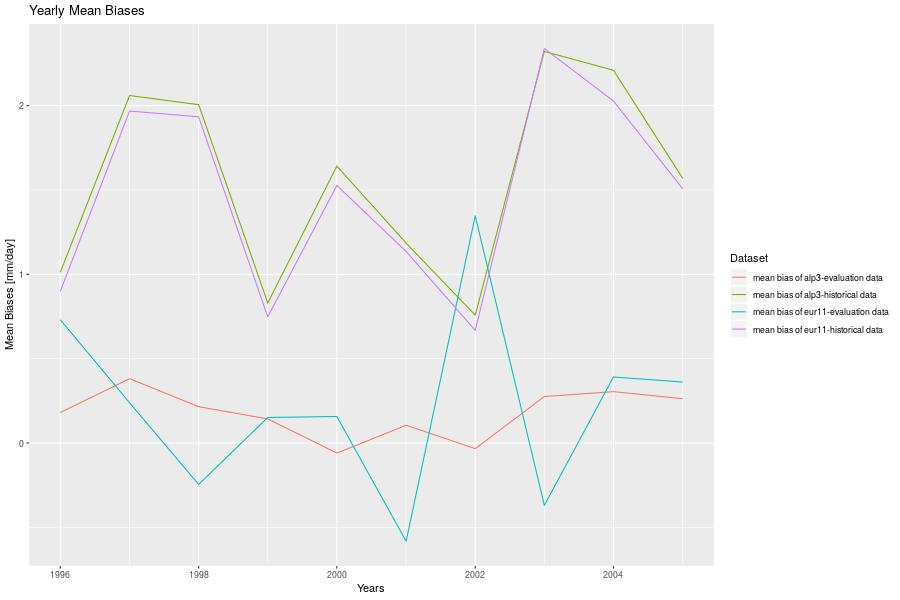
\includegraphics[width=\textwidth]{mean_n/yearly_mean_biases.jpg}
	\caption{Die Biases der gemittelten Differenzen aller vier Datensätze aufgetragen gegen die Zeit}
	\label{fig:yearly_mean_biases}
\end{figure}
Wie man gut in der Abbildung \ref{fig:yearly_mean_biases} erkennen kann, liegt der Bias des evaluation-Datensatzes weit näher bei 0 als die des historicals. Des Weiteren ist gut zu erkennen, dass die Abweichung des Datensatzes ALP-3 betrieben mit den Re-Analysedaten (evaluation) die Beobachtungsdaten gut abbildet und somit ein gutes Klimamodell für den Alpenraum darstellt. Der Bias in diesem Fall ist sehr nahe bei 0. Beide Klimamodelle betrieben mit dem GCM MPI-ESM-LR liefern Ergebnisse, die einen starken Bias in positive Richtung aufweisen, wobei hier kaum noch Unterschiede zwischen EUR-11 und ALP-3 auszumachen sind. Diese Abbildung spricht somit für die Qualität des regionalen Klimamodells, ALP-3 und gegen die Treffsicherheit des globalen Klimamodells.\\
Da der BIAS statistisch gesehen nicht hinreichend aussagekräftig ist, wurden in Abb.\ref{fig:mean_freq_plots} die Häufigkeiten der Abweichungen abgebildet, sowie ein Boxplot in Abb.\ref{fig:mean_boxplots} angelegt, wo zu erkennen ist, dass es einige große Ausreißer gibt. Auf diesen Fakt wird auch in Folge eingegangen, da es über das gesamte Gitter starke Schwankungen der Abweichung gab, welche sich vor allem an den Gebirgskämmen abzeichnete.\\

\begin{figure}[h!]
	\begin{subfigure}{0.49\textwidth}
		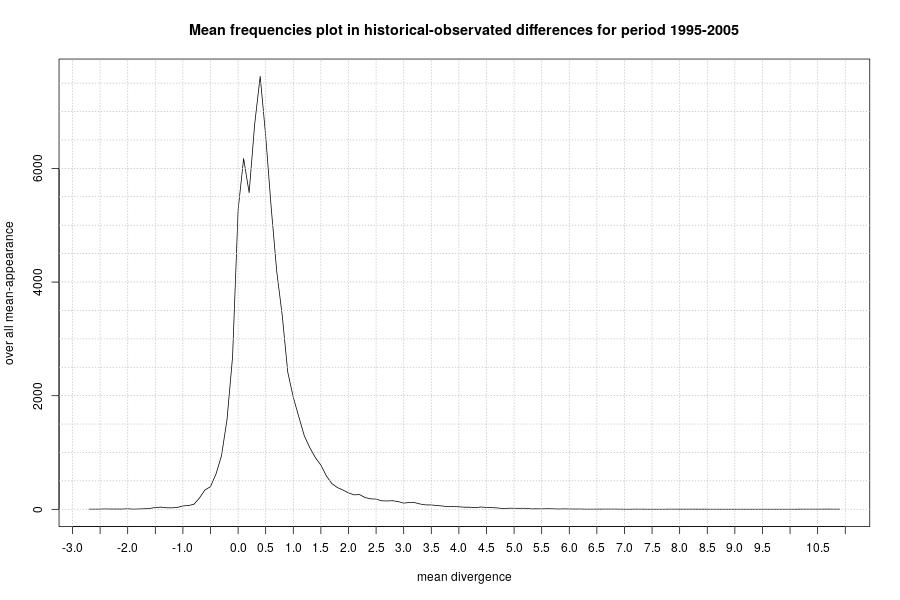
\includegraphics[width=\textwidth]{mean_n/frequenciesdif_mean_hist.jpg}
		\caption{Historical, EUR-11}
	\end{subfigure}
	\begin{subfigure}{0.49\textwidth}
		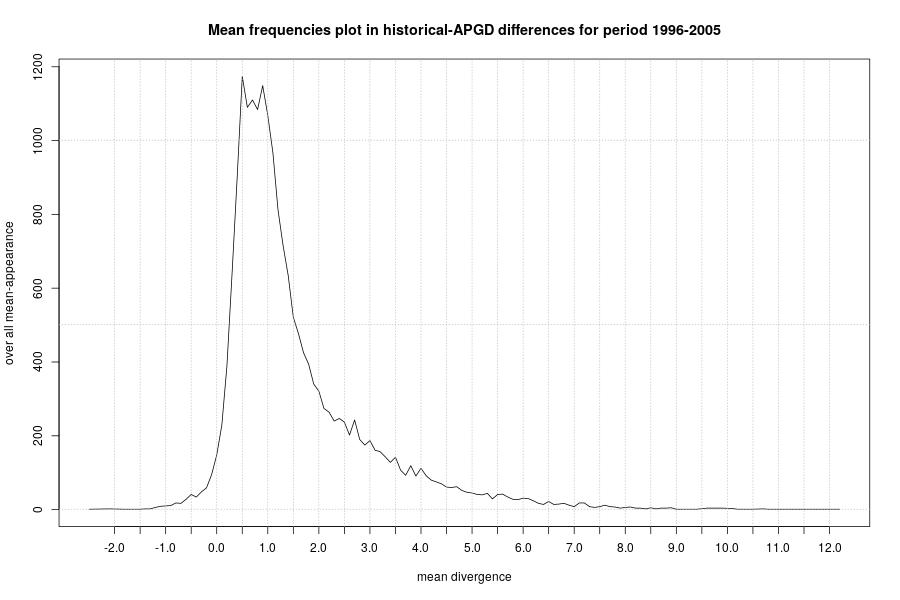
\includegraphics[width=\textwidth]{mean_n/frequenciesdif_mean_hist_apgd.jpg}
		\caption{Historical, ALP-3}
	\end{subfigure}
	\begin{subfigure}{0.49\textwidth}
		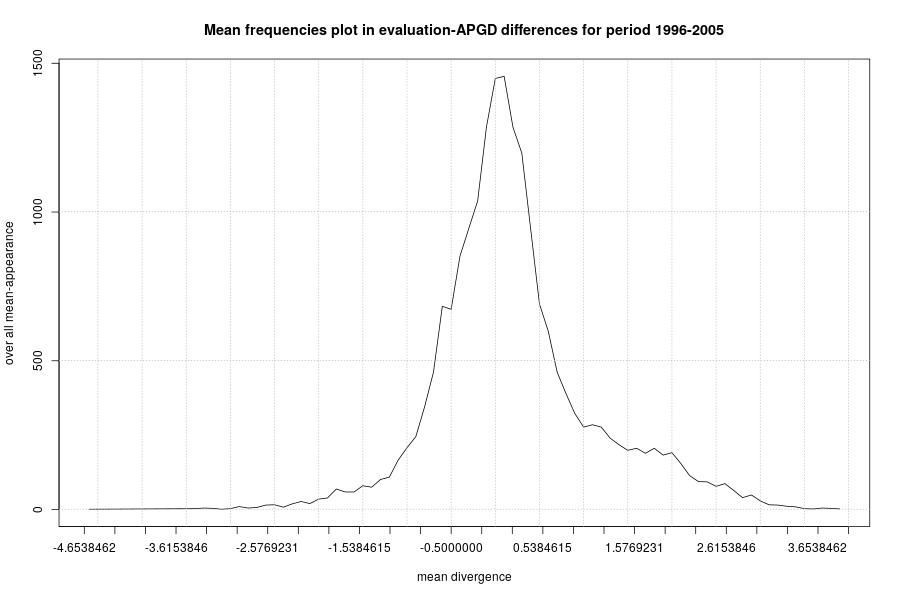
\includegraphics[width=\textwidth]{mean_n/frequenciesdif_mean_eval.jpg}
		\caption{Evaluation, EUR-11}
	\end{subfigure}
	\begin{subfigure}{0.49\textwidth}
		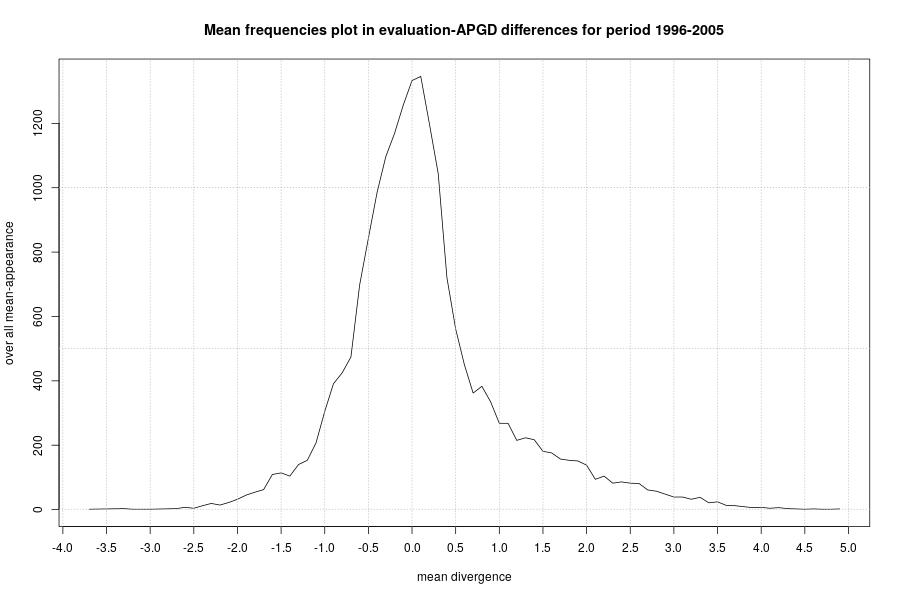
\includegraphics[width=\textwidth]{mean_n/frequenciesdif_mean_eval_apgd.jpg}
		\caption{Evaluation, ALP-3}
	\end{subfigure}
	\caption{Frequency-Plots der Differenzen des jährlichen Mittels des Niederschlags gemittelt über alle Jahre}
	\label{fig:mean_freq_plots}
\end{figure}
\begin{figure}[h!]
	\begin{subfigure}{0.49\textwidth}
		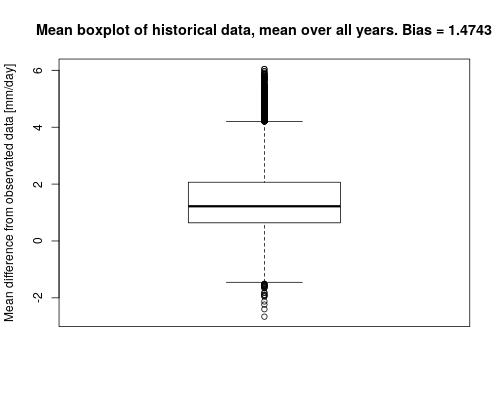
\includegraphics[width=\textwidth]{mean_n/eur_11_mean_historical_boxplot.jpg}
		\caption{Historical, EUR-11}
	\end{subfigure}
	\begin{subfigure}{0.49\textwidth}
		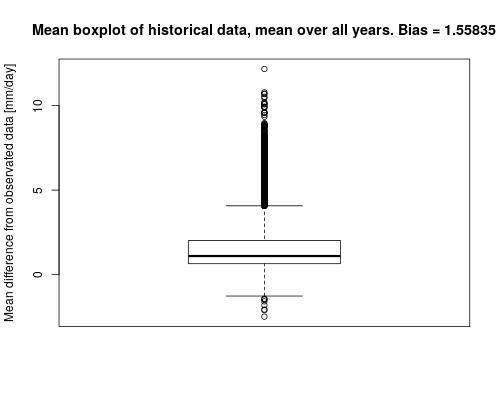
\includegraphics[width=\textwidth]{mean_n/alp3_mean_historical_boxplot.jpg}
		\caption{Historical, ALP-3}
	\end{subfigure}
	\begin{subfigure}{0.49\textwidth}
		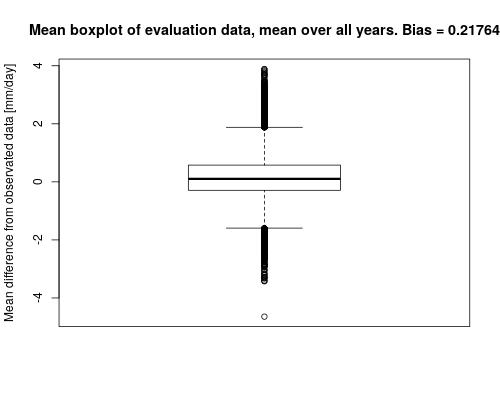
\includegraphics[width=\textwidth]{mean_n/eur_11_mean_evaluation_boxplot.jpg}
		\caption{Evaluation, EUR-11}
	\end{subfigure}
	\begin{subfigure}{0.49\textwidth}
		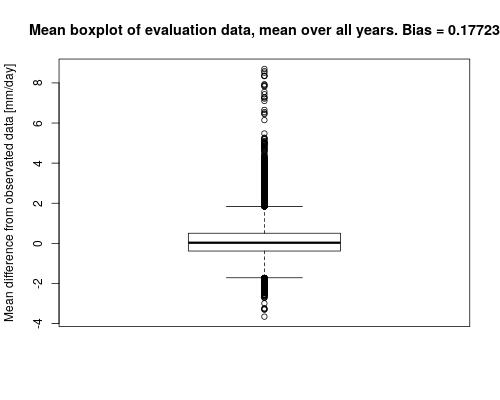
\includegraphics[width=\textwidth]{mean_n/alp3_mean_evaluation_boxplot.jpg}
		\caption{Evaluation, ALP-3}
	\end{subfigure}
	\caption{Box-Plots der Differenzen des jährlichen Mittels des Niederschlags gemittelt über alle Jahre}
	\label{fig:mean_boxplots}
\end{figure}
\begin{figure}[h]
	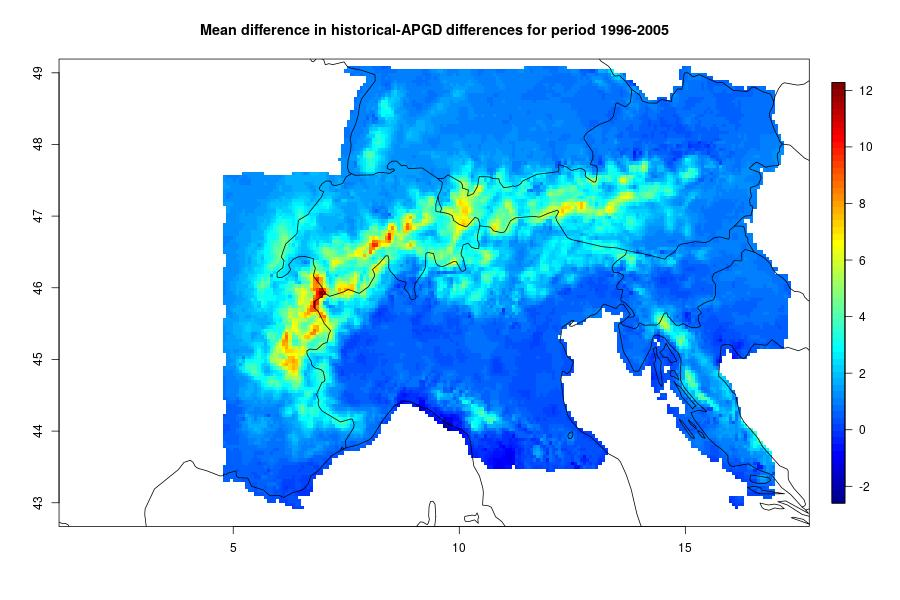
\includegraphics[width=\textwidth]{mean_n/dif_mean_hist_apgd.jpg}
    \caption{Differenzen der jährlichen Mittel, gemittelt über alle Jahre, Datensatz: Historical, ALP-3}
    \label{fig:alp3_dif_hist_mean}
\end{figure}
Um die örtliche Beschaffenheit der größten Abweichungen darzustellen wurden eine Beispielhafte Darstellung gewählt, die die größten mittleren Abweichungen zeigt: der Datensatz Historical im regionalen Klimamodell ALP-3. Diese ist in Abbildung \ref{fig:alp3_dif_hist_mean} abgebildet.
Wie man gut in der Abbildung erkennen kann, ist im Allgemeinen über den orthographisch gediegenen Gegenden die Abweichung vom Beobachtungsdatensatz gering. Es ist gut ersichtlich, dass die Abweichungen in überwiegend gebirgigen Gegenden größer sind. Wie auch in den Abbildungen \ref{fig:mean_freq_plots} zu sehen ist, überwiegt eine Abweichung von $0.5-1$. Die Kurve ist auch leicht ins rechte verschoben - dies bedeutet dass mehr Niederschlage simuliert wurde als es tatsächlich gab. Dies könnte somit eine Schwäche des Klimamodells darstellen, da sich dieses Muster auch im den anderen Datensätzen abzeichnet, wie im folgenden Kapitel erkenntlich gemacht werden soll. \newpage

\section{Beobachtungen eines Jahres: 2002} \label{section:2002}
Das Jahr 2002 wurde gewählt, da sich mit diesem Jahr die nahezu gleichbleibende Differenzen-Verteilung am besten darstellen lässt, wie man in Abbildung \ref{fig:yearly_mean_biases} erkennen kann. In diesem Kapitel soll es darum gehen, die Ortographie bzw. die örtliche Verteilung der Differenzen näher zu betrachten. Dazu wurden zunächst die Abweichungen des Jahresmittels bildlich dargestellt: Abb. \ref{fig:dif_mean_2002_1} und \ref{fig:dif_mean_2002_2}. Wie man erkennen kann, häufen sich Analog zu den Differenzen, gemittelt über alle Jahre die Abweichungen besonders in den orthographisch hervorstechenden Gebieten, in den Ebenen scheint die Übereinstimmung gut zu sein.\\
\begin{figure}[h]
		\begin{subfigure}{0.49\textwidth}
			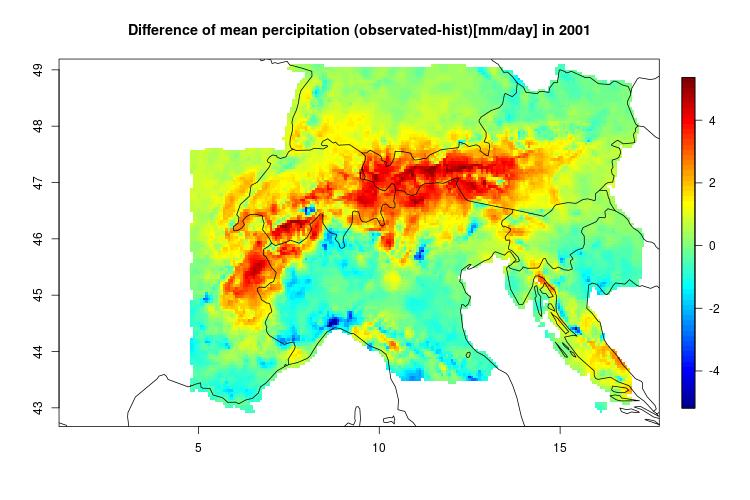
\includegraphics[width=\textwidth]{mean_n/2002dif_mprs_hist-obs.jpg}
			\caption{Historical, EUR-11}
			\label{fig:dif_mean_2002:eur11_hist}
		\end{subfigure}
		\begin{subfigure}{0.49\textwidth}
			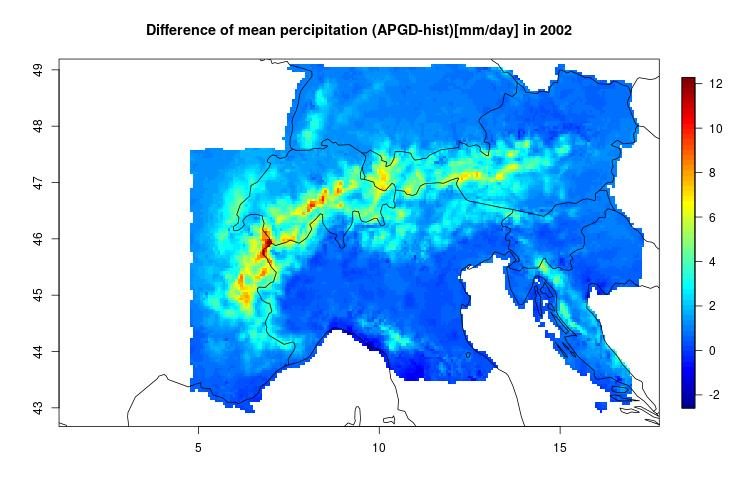
\includegraphics[width=\textwidth]{mean_n/2002dif_mprs_alp3hist-apgd.jpg}
			\caption{Historical, ALP-3}
			\label{fig:dif_mean_2002:alp3_hist}
		\end{subfigure}
	\caption{Differenzen des jährlichen Mittels über den Niederschlag im Jahr 2002}
	\label{fig:dif_mean_2002_1}
\end{figure}
\begin{figure}
		\begin{subfigure}{0.49\textwidth}
			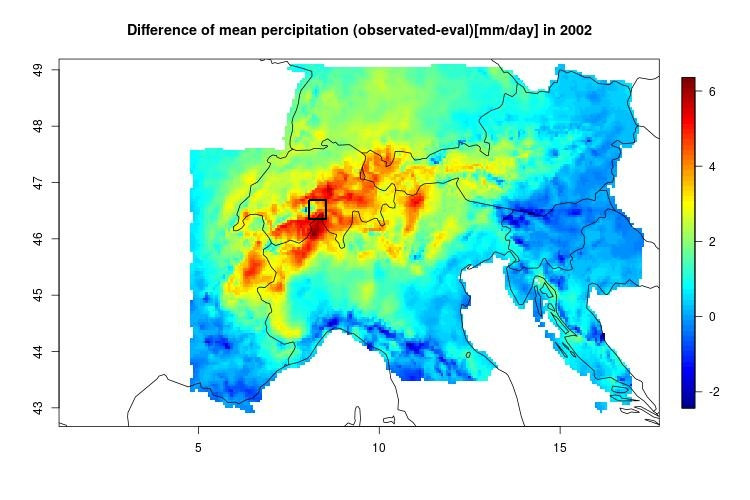
\includegraphics[width=\textwidth]{mean_n/2002dif_mprs_eval-obs.jpg}
			\caption{Evaluation, EUR-11}
			\label{fig:dif_mean_2002:eur11_eval}
		\end{subfigure}
		\begin{subfigure}{0.49\textwidth}
			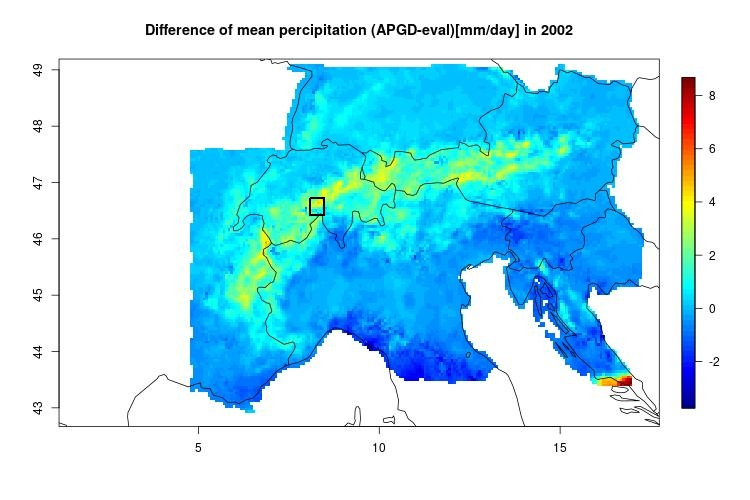
\includegraphics[width=\textwidth]{mean_n/2002dif_mprs_alp3eval-apgd.jpg}
			\caption{Evaluation, ALP-3}
			\label{fig:dif_mean_2002:alp3_eval}
		\end{subfigure}
	\caption{Differenzen des jährlichen Mittels über den Niederschlag im Jahr 2002}
	\label{fig:dif_mean_2002_2}
\end{figure}
\begin{figure}
	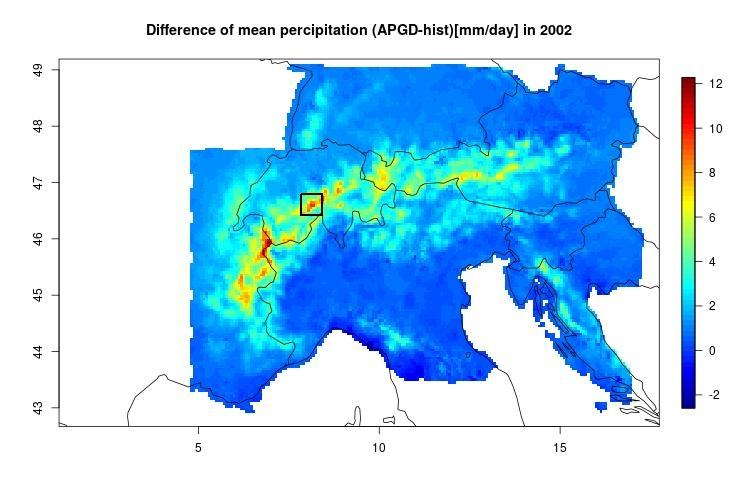
\includegraphics[width=\textwidth]{mean_n/decision_plot_hist_alp3_2002.jpg}
	\caption{Der Bereich in dem die Abweichungen für alle Datensätze am größten ist, gekennzeichnet mit der Niederschlagsmenge 20mm/day - dunkelrot}
	\label{fig:decision_mean_2002}
\end{figure}

Wie in den Abbildungen \ref{fig:dif_mean_2002_1} und \ref{fig:dif_mean_2002_2} zu erkennen ist bleibt in einem gewissen Bereich die Abweichungen über alle Datensätze am größten.Deshalb wurde dieser in Folge gesondert betrachtet. Der Bereich wurde in der Abbildung \ref{fig:decision_mean_2002} als dunkelrotes Rechteck gekennzeichnet (mit 20 mm/day).\\
Dieser Bereich wurde in allen Modell-Datensätzen ausgeschnitten und im Jahr 2002 über dessen Fläche gemittelt, somit ergab sich aus dem feinen Gitter ein Mittelwert für jeden Tag für jeden Datensatz. Von diesen Werten wurden dann die ebenfalls Flächen-gemittelten Beobachtungsdaten (APGD) abgezogen und daraus ergab sich das Diagramm in Abb.\ref{fig:diff_2002}.\\
\begin{figure}[h]
	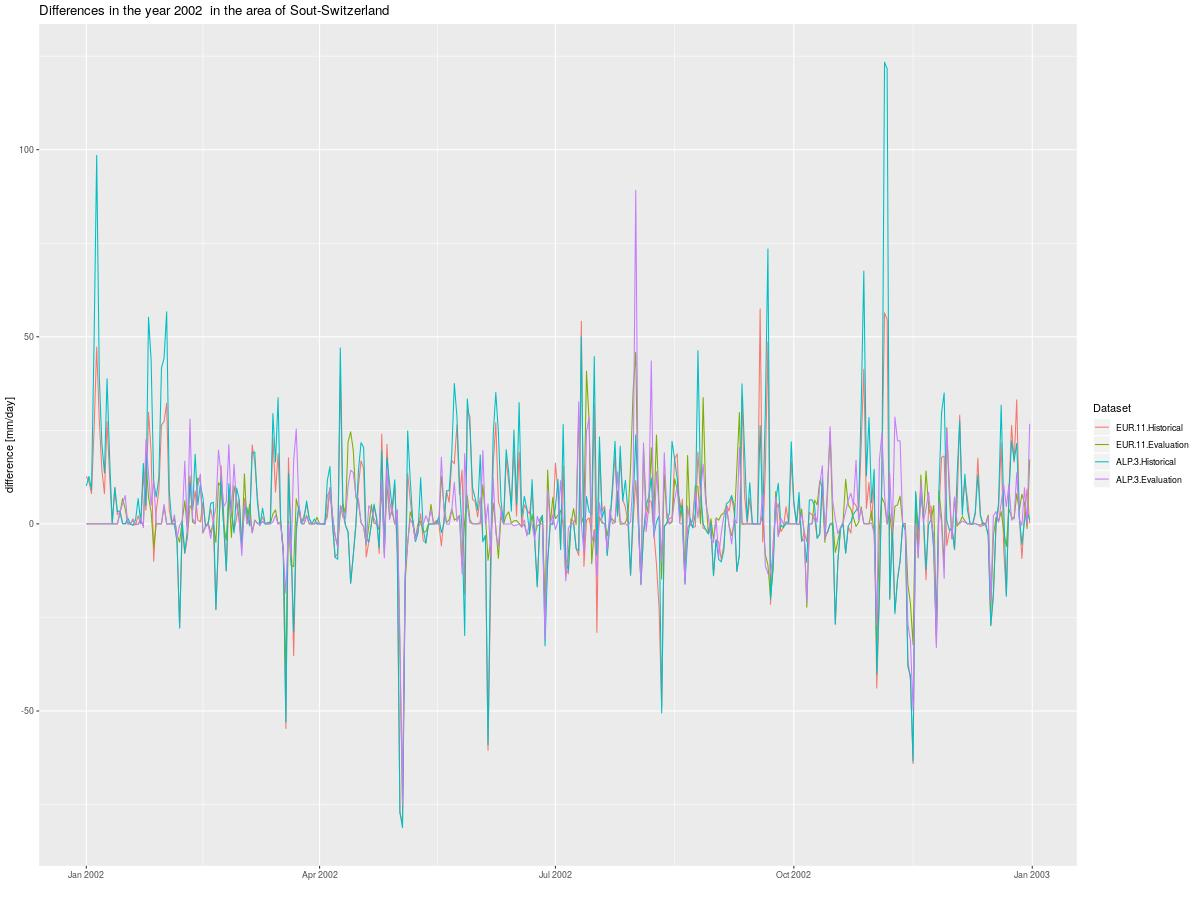
\includegraphics[width=\textwidth]{mean_n/differences_2002.jpg}
	\caption{Die Differenzen für den in Abb. \ref{fig:decision_mean_2002} angegebenen Bereich im Jahr 2002. Es muss beachtet werden, dass hier die tägliche Inkonsistenz betrachtet wird, dies ist nicht ein Fehler des Modells.}
	\label{fig:diff_2002}
\end{figure}\\
Man sieht in Abb.\ref{fig:diff_2002}, dass die Abweichungen über das Jahr verteilt stark fluktuieren. Beachtenswert ist dabei, dass die Ausschläge der Kurven für den ALP-3 Datensatz deutlich größer sind und somit auch die Abweichungen. Diese sind zudem auffallend in das Positive verschoben. Auch gut zu erkennen ist, dass die Kurvenform der beiden Historical bzw. Evaluation - Datensätzen nahezu identisch sind, was auf Fehler in den Antriebsdaten rückzuführen ist. Da die Ausschläge gemittelt über das ganze Gebiet (vgl. Abb.\ref{fig:mean_boxplots} und Abb.\ref{fig:mean_freq_plots}) für den ALP-3 Datensatz deutlich besser (näher bei $0$) sind ist es in diesem gesondert betrachteten Gebiet wahrscheinlich zu einem Overfitting des Modells gekommen und die extremen Ausschläge sind Fluktuationen die daraus resultieren. Um nun in Folge die Anpassung der beiden Modelle EUR-11 und ALP-3 an die Regenereignisse besser untersuchen zu können wurden die beiden Datensätze mit den größten Abweichungen (Historical aus EUR-11 und ALP-3) in Abb.\ref{fig:precip_2002} dargestellt.\\

\begin{figure}[h]
	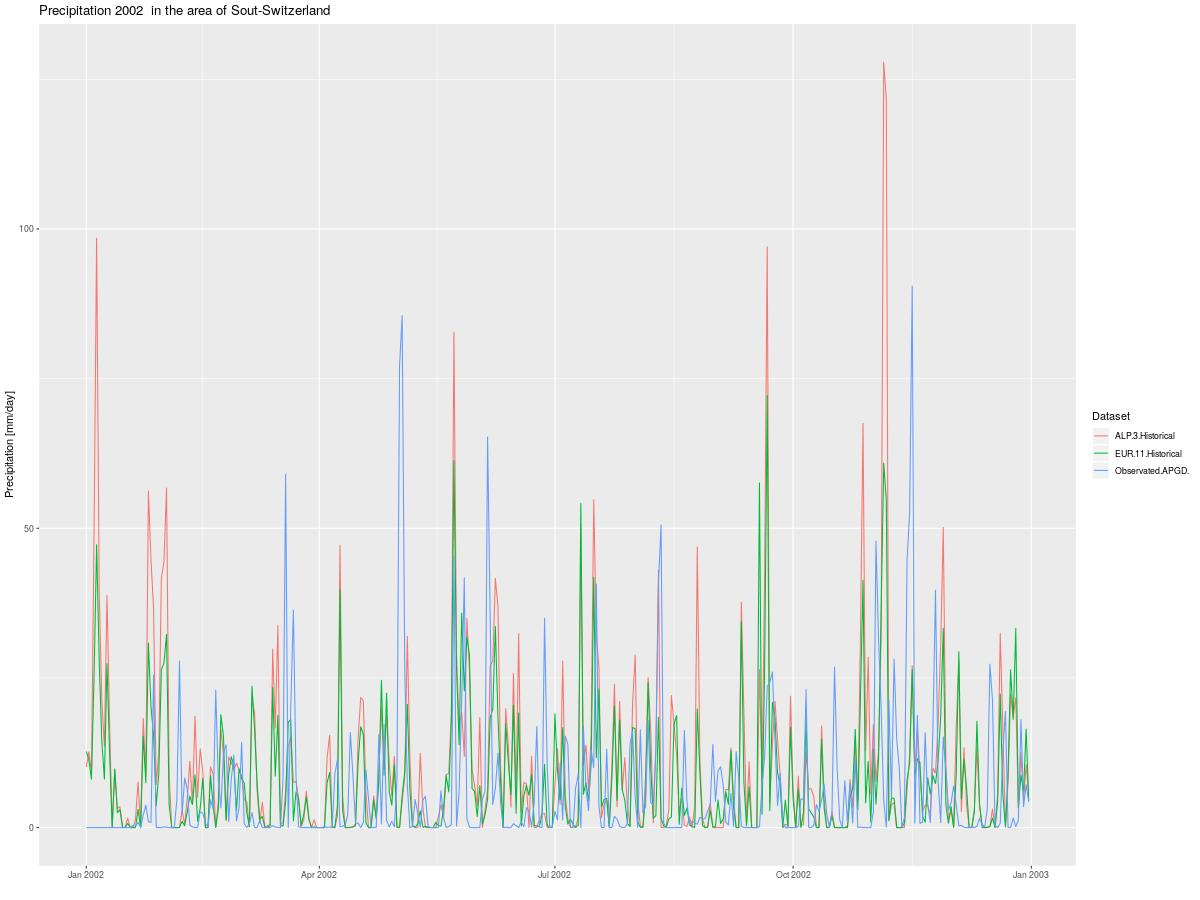
\includegraphics[width=0.90\textwidth]{mean_n/historical_2002.jpg}
	\caption{Niederschlag im Jahr 2002 fuür den in Abb.\ref{fig:decision_mean_2002} gekennzeichneten Bereich aus den Datensätzen Historical von ALP-3 bzw. EUR-11 gegen die Beobachtungsdaten aus APGD}
	\label{fig:precip_2002}
\end{figure}
\begin{figure}[h]
	\begin{subfigure}{0.49\textwidth}
		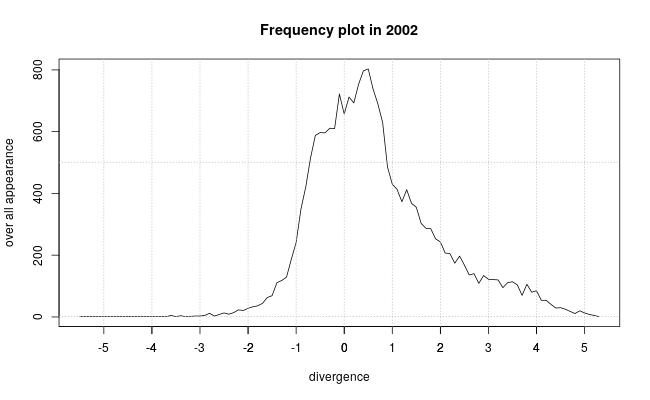
\includegraphics[width=\textwidth]{mean_n/2002frequenciesdif_mprs_hist-obs.jpg}
		\caption{EUR-11, Historical}
	\end{subfigure}
	\begin{subfigure}{0.49\textwidth}
		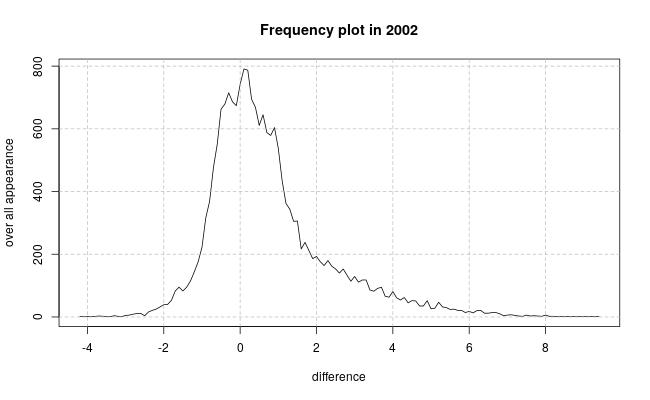
\includegraphics[width=\textwidth]{mean_n/2002frequenciesdif_mprs_alp3hist-apgd.jpg}
		\caption{ALP-3, Historical}
	\end{subfigure}
	\caption{Häufigkeit gewisser Abweichungen für das gemittelte Jahr 2002 in den beiden Historical-Datensätzen (betrachtetes Gebiet: \underline{gesamter} Alpenraum)}
	\label{fig:freq_2002}
\end{figure}
\newpage

In der Abb. \ref{fig:precip_2002} liegen die im regionalen Klimamodell (ALP-3) die vorhergesagten Niederschlags\underline{mengen} für Extremniederschläge z.B. im Mai 2002 um einiges näher an den Beobachteten. Es werden jedoch auch manche Niederschlagsereignisse schlichtweg überschätzt, was sich dann im Gesamtbild schlecht auswirkt (vgl.\ref{fig:freq_2002}: die Kurve ist deutlich ins Positive verschoben.\\
Das Klimamodell welches die Konvektion nicht simuliert (EUR-11) scheint dauernd eine gewisse Fluktuation im Niederschlag zu errechnen ohne gezielt Starkregenereignisse zu reproduzieren. Dies ist gut im Bereich April 2002 in der Abb. \ref{fig:precip_2002} zu erkennen: Die Fluktuationen scheinen gewissermaßen ständig aufzutreten. Das ist auf die Parametrisierung der Konvektion zurückzuführen. Da dadurch auch keine längeren Regenpausen vorkommen können ist dies ein großes Manko in der Vorhersagekraft von diesen Modellen für die zukünftige Entwicklung des Wetter auf regionaler Ebene (siehe ''Bias Correction, Quantile Mapping, and Downscaling: Revisiting the Inflation Issue'' von D.Maraun \cite{biasMaraun}). \\
Das Konvektion-simulierende Klimamodell ALP-3 scheint besonders im Winter und im Herbst Niederschlagsextrema zu überschätzen. Im Sommer  bzw. Frühling stimmen die Daten relativ gut überein. Manche Extrema sind zwar zeitlich verschoben, jedoch muss bemerkt werden, dass die historischen Tage nichts mit den simulierten Tage im Klimamodell gemein haben, somit darf die zeitliche Verteilung nicht zu genau genommen werden. Sondern es muss eine gewisse Toleranz, wann ein Starkregenereignis eintritt mit-einberechnet werden.\\
\section{Zusammenfassung}
Wie in diesem Kapitel gezeigt wurde, kann der Mittelwert alleine nicht zur Evaluierung eines Klimamodells herangezogen werden, da dadurch die Extremwetter aus den Daten ausgemittelt werden, und auch der Mittelwert des Niederschlags nicht das Klima einer Region beschreibt. Nichtsdestotrotz gibt der Mittelwert (jährlich und alljährlich) einen guten Aufschluss darüber, wo die größten Abweichungen herrschen (siehe Kapitel \ref{section:2002}). Jedoch sobald man ein Jahr oder auch die gesamte Zeitspanne genauer betrachten will steht man bald an dem Problem an, dass die simulierten Tage nicht direkt mit den historischen Tagen in Verbindung gebracht werden dürfen. Um nun diese tägliche Inkonsistenz aus der Betrachtung Außenvorzulassen soll im nächsten Kapitel auf die alljährlichen Extremwettererscheinungen eingegangen werden.

